% -----------------------------------------------------------------------------
% Project: PhD KAPPA
% File: kappa.Rnw (root file)
% Author: Alessio Crippa
% Template: based on the tex code written by Andrea Discacciati
%           url: https://github.com/anddis/phd-thesis
%
% Purpose: Root Rnw file, compile this to typeset the kappa!
% -----------------------------------------------------------------------------



% If you get the following error:
%  Error in ensurePackageSymlink(source, target) :
% run the next line, an then restart your R session
% unlink("packrat/lib-R", recursive = TRUE)


% Class
\documentclass[11pt,a4paper,twoside,openany]{book}\usepackage{knitr}

% Packages
\usepackage[english]{babel}
\usepackage{amsfonts}
\usepackage{amsmath}
\usepackage{mathtools}
\usepackage{threeparttable}
\usepackage{adjustbox}
\usepackage{natbib}
\usepackage{graphicx}
\usepackage{flafter}
\usepackage{fancyhdr}
\usepackage{textcomp}
\usepackage[utf8]{inputenc}
\usepackage{setspace}
\usepackage[pdftex,
            pdfauthor={Alessio Crippa},
            pdftitle={Novel methods for dose--response meta-analysis},
            pdfcreator={LaTeX2e}]{hyperref}
\usepackage[%showframe,
			headheight=13.6pt,
			%headsep=,
			%footskip=,
			bindingoffset=0cm,%print=.5cm, web=0cm
			left=3cm,  %print=2cm, web=3cm
			bottom=3cm, %print=3cm, web=3cm
			top=3cm, %print=3cm, web=3cm,
			right=3cm]{geometry} %print=3.5cm, web=3cm
\usepackage{enumerate, mdwlist}
\usepackage{etoolbox}
\usepackage{tabularx}
\usepackage{rotating}
\usepackage[font={small}]{caption}
\usepackage{chngcntr}
\usepackage{booktabs}
\counterwithout{footnote}{chapter}

%---begin see http://www.khirevich.com/latex/font/
\usepackage[activate={true,nocompatibility},final,tracking=true,kerning=true,spacing=true,factor=1100, stretch=10,shrink=10]{microtype}
% remove warning
\microtypecontext{spacing = nonfrench}
\usepackage[T1]{fontenc}
% remove warning
\global\expandafter\let\csname ver@amsfonts.sty\endcsname\relax
% remove issue related to interwordspace
\setlength{\emergencystretch}{10pt}
\usepackage[bitstream-charter]{mathdesign}
\usepackage{sectsty}
	\chapterfont{\usefont{T1}{qhv}{b}{n}\selectfont\huge}
\usepackage{titlesec}

% ---------------------------------------------------------
% Project: PhD KAPPA
% File: _titlesec.tex
% Author: Andrea Discacciati
%
% Purpose: Headings format
%			(see titlesec package)
% ---------------------------------------------------------

\titleformat{\section}[hang]{
    \usefont{OT1}{qhv}{bx}{n}\selectfont}
    {} 
    {0em}
    {\hspace{-0.4pt}\Large \thesection\hspace{0.6em}}
\titleformat{\subsection}[hang]{
    \usefont{OT1}{qhv}{bx}{n}\selectfont}
    {} 
    {0em}
    {\hspace{-4pt} \thesubsection\hspace{0.6em}}
\titleformat{\subsubsection}[hang]{
    \usefont{OT1}{qhv}{bx}{n}\selectfont}
    {} 
    {0em}
    {\normalsize}
\usepackage{tocloft}

% ---------------------------------------------------------
% Project: PhD KAPPA
% File: _tocloft.tex
% Author: Andrea Discacciati
%
% Purpose: Table of Contents, 
%			List of Figures, List of Tables format
%			(see tocloft package)
% ---------------------------------------------------------

\renewcommand{\cfttoctitlefont} % ToC title
             {\usefont{T1}{qhv}{b}{n}\selectfont\huge}
\renewcommand{\cftchapfont} % chapter titles
             {\usefont{T1}{qhv}{b}{n}\selectfont}
\renewcommand{\cftsecfont} % section titles
             {\usefont{T1}{bch}{m}{n}\selectfont}
\renewcommand{\cftsubsecfont} % subsection titles
             {\usefont{T1}{bch}{m}{n}\selectfont} 
\renewcommand{\cftchappagefont} % chapter page numbers
             {\usefont{T1}{bch}{b}{n}\selectfont}
\renewcommand{\cftsecpagefont} % section page numbers
             {\cftsecfont} 
\renewcommand{\cftsubsecpagefont} % subsection page numbers
             {\cftsubsecfont}
             
\renewcommand{\cftloftitlefont} % LoF title
             {\usefont{T1}{qhv}{b}{n}\selectfont\huge}
\renewcommand{\cftfigfont} % Figures titles
             {\usefont{T1}{bch}{m}{n}\selectfont}
             
\renewcommand{\cftlottitlefont} % LoT title
             {\usefont{T1}{qhv}{b}{n}\selectfont\huge}
\renewcommand{\cfttabfont} % Tables titles
             {\usefont{T1}{bch}{m}{n}\selectfont}
%---end see http://www.khirevich.com/latex/font/

% Header / footer

% ---------------------------------------------------------
% Project: PhD KAPPA
% File: _fancyhdr.tex
% Author: Alessio Crippa
% based on the template written by Andrea Discacciati
%
% Purpose: Header and footer settings
%			(see fancyhdr package)
% ---------------------------------------------------------

\pagestyle{fancy}
\renewcommand{\chaptermark}[1]{%
 \markboth{{\thechapter.\ #1}}{}}

\fancypagestyle{plain}{%
  \fancyhf{}%
  \renewcommand{\headrulewidth}{0pt}%
  \fancyhf[lef,rof]{}%
  %\fancyhead[LE,RO]{\thepage}
}

\fancypagestyle{frontmatter}{%
  \renewcommand{\headrulewidth}{0pt} 
  \renewcommand{\footrulewidth}{0pt}
  \fancyhf{}% Clear header/footer
  \fancyhead[LE,RO]{}
}

\fancypagestyle{nothing}{%
  \renewcommand{\headrulewidth}{0pt} 
  \renewcommand{\footrulewidth}{0pt}
  \fancyhf{}% Clear header/footer
  \fancyhead[LE,RO]{}%
}

\fancypagestyle{mainmatter}{%
  \renewcommand{\headrulewidth}{.4pt}
  \renewcommand{\footrulewidth}{0pt}
  \fancyhf{}% Clear header/footer
  \fancyhead[LE,RO]{\thepage}
  \fancyhead[RE,LO]{\nouppercase \leftmark}
}

	
% See 'writing a thesis with latex' p25 
% Writes nothing on empty pages
\makeatletter
\def\cleardoublepage{\clearpage\if@twoside
\ifodd\c@page
\else\hbox{}\thispagestyle{empty}\newpage
\if@twocolumn\hbox{}\newpage\fi\fi\fi}
\makeatother

% Substitutions (%examples)
%\newcommand{\rveplot}{decorrelated-residuals--versus--exposure plot}
%\newcommand{\kgmsq}{kg$\times$m\textsuperscript{$-2$}}

\defcitealias{crippadosresmeta2016}{Paper~I}	
\defcitealias{discacciati2015goodness}{Paper~II}	
\defcitealias{crippa2016new}{Paper~III}	
\defcitealias{crippa2018pointwise}{Paper~IV}	
\defcitealias{crippa2018one}{Paper~V}	

%\doublespacing 
\onehalfspacing

\allowdisplaybreaks

\renewcommand{\sfdefault}{qhv}
\newcommand*{\LargerCdot}{\raisebox{-0.25ex}{\scalebox{1.2}{$\cdot$}}}

\DeclareMathOperator{\R}{\textsf{R}}
\DeclareMathOperator{\Var}{Var}
\DeclareMathOperator{\SE}{SE}
\DeclareMathOperator{\Cov}{Cov} 
\DeclareMathOperator{\diag}{diag} 
\DeclareMathOperator{\N}{N} 
\DeclareMathOperator{\E}{E}
\DeclareMathOperator{\logit}{logit} 
\DeclareMathOperator{\df}{df} 
\hyphenation{logRRs}
\hyphenation{logRR}

\addto\captionsenglish{%
  \renewcommand{\bibname}{References}%
}

%\includeonly{abstract, results, introduction, background, aims, discussion, conclusions }

%--- Kappa starts here! ---%
\IfFileExists{upquote.sty}{\usepackage{upquote}}{}
\begin{document}

% Front matter
\frontmatter
\pagestyle{nothing}

% ---------------------------------------------------------
% Project: PhD KAPPA
% File: titlepage.tex
% Author: Alessio Crippa
% based on the template written by Andrea Discacciati
%
% Purpose: Custom title page + ISBN/copyright page
% ---------------------------------------------------------

\begin{titlepage}
\newgeometry{margin=4cm}
\begin{center}
\large
From the Department of Public Health Sciences \\
Karolinska Institutet, Stockholm, Sweden        
\vfill
\Large
\textbf{\textsf{NOVEL METHODS FOR DOSE-RESPONSE META-ANALYSIS}}
\vfill
\Large
Alessio Crippa
\vfill

\includegraphics[width=0.8\textwidth]{figures/ki-logo_pos}
\vfill
\large
Stockholm 2018        
\end{center}
\restoregeometry
\end{titlepage}

\newpage
\null
\vfill
\noindent All published papers reproduced with permission \\
%Cover illustration ``Portraits of sophistication'' by Lamai McCartan \\
Published by Karolinska Institutet \\
\bigskip
Printed by E-Print AB 2018 \\
Edited in R using knitr \\
\textcopyright Alessio Crippa, 2018 \\
ISBN <include number>
\newpage

% ---------------------------------------------------------
% Project: PhD KAPPA
% File: spikblad.tex
% Author: Alessio Crippa
% based on the template written by Andrea Discacciati
%
% Purpose: Spikblad
% ---------------------------------------------------------
\null
\vspace{1.5cm}
\noindent{\Large \textsf{NOVEL METHODS FOR DOSE-RESPONSE META-ANALYSIS} \vspace{1cm}}\\
\noindent{\Large \textsf{THESIS FOR DOCTORAL DEGREE (Ph.D.)} \vspace{.5cm}}\\
By \vspace{.5cm} \\
{\Large \textbf{\textsf{Alessio Crippa}} \vspace{2cm}}\\
\begin{minipage}[t]{6.2cm}
\singlespacing
{\small
\textit{Principal supervisor:}\\
Associate Professor Nicola Orsini \\
Karolinska Institutet \\
\bigskip
Department of Public Health Sciences \\
\textit{Co-supervisor:}\\
Professor Alicja Wolk \\
Karolinska Institutet \\
\medskip
Institute of Environmental Medicine \\
Professor Matteo Bottai \\
Karolinska Institutet \\
\medskip
Institute of Environmental Medicine \\
Professor Donna Spiegelman \\
Harvard T.H. Chan School of Public Health \\
Department of Epidemiology
}
\end{minipage}
\hspace{1.5cm}
\begin{minipage}[t]{8.1cm}
\singlespacing
{\small
\textit{Opponent:}\\
Professor Christopher H. Schmid \\
Brown University \\
Center for Evidence Based Medicine\bigskip \\
\textit{Examination board:}\\
Associate Professor Nele Brusselaers \\
Karolinska Institutet \\
Department of Microbiology, Tumor and Cell Biology \medskip \\
Associate Professor Antonio Gasparrini \\
London School of Hygiene and Tropical Medicine \\
Department of Social $\&$ Environmental Health Research\medskip \\
Professor Paul Lambert \\
University of Leicester \\
Department of Health Sciences
}
\end{minipage}
\cleardoublepage

% ---------------------------------------------------------
% Project: PhD KAPPA
% File: dedication.tex
% Author: Alessio Crippa
% based on the template written by Andrea Discacciati
%
% Purpose: Dedication
% ---------------------------------------------------------

\begin{flushright}
%http://pubmedcentralcanada.ca/pmcc/articles/PMC2550765/pdf/bmj00610-0065.pdf
\null\vspace{\stretch{1}}
\textit{``The function of the expert reviewer is not to be more right than other people, \\
but to be wrong for more sophisticated reasons.''} \\
---Iain Chalmers and Douglas G. Altman \\ 
\textit{Systematic Reviews}, 1995
\vspace{\stretch{2}}\null
\end{flushright}


\iffalse
\begin{flushright}
\null\vspace{\stretch{1}}
\textit{``If I have seen further, it is by standing on the shoulders of giants.''} \\
---Isaac Newton
\vspace{\stretch{2}}\null
\end{flushright}
\fi
\cleardoublepage 
\pagestyle{frontmatter}

% ---------------------------------------------------------
% Project: PhD KAPPA
% File: abstract.tex
% Author: Andrea Discacciati
%
% Purpose: Abstract frontmatter
% ---------------------------------------------------------


\noindent {\Large \textsf{\textbf{{Abstract}}}
\bigskip
%\chapter*{Abstract}
\small
\par Dose--response meta-analysis is a statistical procedure for combining and contrasting the evidence on the association between a continuous exposure and the risk of a health outcome. Several papers refined selected aspects of the methodology, such as implementation of flexible strategies and extensions to multivariate meta-analysis. However, there were still several relevant questions that needed to be addressed. This thesis aims to address these issues by developing and implementing new strategies and ad-hoc measures (\citetalias{crippadosresmeta2016}), including tools for evaluating the goodness-of-fit (\citetalias{discacciati2015goodness}), a new measure for quantifying the impact of heterogeneity (\citetalias{crippa2016new}), a strategy to deal with differences in the exposure range across studies (\citetalias{crippa2018pointwise}), and a one-stage approach to estimate complex models without excluding relevant studies (\citetalias{crippa2018one}).

In \citetalias{crippadosresmeta2016}, we described the implementation of the main aspects of the methodology in the \texttt{dosresmeta} $\R$ package available on CRAN. Dedicated functions was written to facilitate specific tasks such as definition of the design matrix and prediction of the pooled results. We illustrated how to estimate both linear and non-linear curves, conduct test of hypotheses, and present the results in a tabular and grapichal format using summarized data on alcohol intake and colorectal cancer risk.
 
In \citetalias{discacciati2015goodness}, we discussed how to evaluate the goodness-of-fit. The proposed solutions consist of descriptive measures to summarize the agreement between fitted and observed data (the deviance and the coefficient of determination), and graphical tools to visualize the fit of the model (decorrelated residuals-versus-exposure plot). A reanalysis of two published meta-analyses exemplified how these tools can improve the practice of quantitative synthesis of aggregated dose--response data. 

In \citetalias{crippa2016new}, we proposed and characterized a new measure, $R_b$, to quantify the proportion of the variance of the pooled estimate attributable to the between-study heterogeneity. Contrary to the available measures of heterogeneity, $R_b$ does not make any assumption about the distribution of the within-study error variances, nor does it require specification of a typical value for these quantities. The performance of the proposed measure was evaluated in an extensive simulation study. We demonstrated how to present and interpret the $R_b$ re-analyzing three published meta-analyses.

In \citetalias{crippa2018pointwise}, we extended a point-wise approach to dose--response meta-analysis of aggregated data. The strategy consists of combining predicted relative risks for a fine grid of exposure values based on potentially different dose--response models. A point-wise approach can improve the flexibility in modeling the study-specific curves and may limit the impact of extrapolation by predicting the study-specific relative risk based on the observe exposure range. We illustrated the methodology using both individual and aggregated participant data.

In \citetalias{crippa2018one}, we formalized a one-stage approach for dose--response meta-analysis in terms of a linear mixed model. We explained the main aspects of the methodology and how to extend the measures typically presented in a two-stage analysis. Using both hypothetical and real data, we showed how the one-stage approach can facilitate investigation the impact of heterogeneity over the exposure range, model comparison, and prediction of individual dose--response associations. The main advantage is that flexible curves can be estimated regardless of the number of data-points in the individual analyses.

In conclusion, the methods presented in this thesis enrich the set of tools available for applying dose--response meta-analyses and for addressing specific questions including goodness-of-fit evaluation (\citetalias{discacciati2015goodness}) and quantification of heterogeneity (\citetalias{crippa2016new}). In addition, we presented alternative models for pooling results in case of heterogeneous exposure range (\citetalias{crippa2018pointwise}) and for estimating complex models without excluding relevant studies (\citetalias{crippa2018one}). The proposed methods have been illustrated using real data and implemented in the \texttt{dosresmeta} and \texttt{hetmeta} $\R$ packages available on CRAN (\citetalias{crippadosresmeta2016}). 

\normalsize
\cleardoublepage

% ---------------------------------------------------------
% Project: PhD KAPPA
% File: publications.tex
% Author: Alessio Crippa
% based on the template written by Andrea Discacciati
%
% Purpose: List of publications + related publications
% ---------------------------------------------------------

\chapter*{List of publications}

\begin{enumerate}[I.]
\item Alessio~Crippa, and Nicola~Orsini \\ \textbf{Multivariate dose--response meta-analysis: the dosresmeta R Package} \\ \textit{Journal of Statistical Software, Code Snippets} 2016; 72(1), 1--15
\item Andrea~Discacciati, Alessio~Crippa, and Nicola~Orsini \\ \textbf{Goodness of fit tools for dose--response meta-analysis of binary outcomes} \\ \textit{Research Synthesis Methods} 2015
\item Alessio~Crippa, Polyna~Khudyakov, Molin~Wang, Nicola~Orsini, and Donna~Spiegelman \\ \textbf{A new measure of between-studies heterogeneity in meta-analysis} \\ \textit{Statistics in medicine} 2016; 35(21), 3661--75
\item Alessio~Crippa, Ilias~Thomas, and Nicola~Orsini \\ \textbf{A pointwise approach to dose-response meta-analysis of aggregated data} \\ \textit{Manuscript} 2018
\item Alessio~Crippa, Andrea~Discacciati, Matteo~Bottai, Alicja~Wolk, and Nicola~Orsini \\ \textbf{One-stage dose--response meta-analysis for aggregated data} \\ \textit{Manuscript} 2018
\end{enumerate}
\vspace{1.5cm}
\noindent{The articles will be referred to in the text by their Roman numerals, and are reproduced in full at the end of the thesis.}

\chapter*{Related publications}
\begin{itemize}
\item Ehimen~C.~Aneni, Alessio~Crippa, Chukwuemeka~U.~Osondu, Javier~Valero‐Elizondo, Adnan~Younus, Khurram~Nasir, and Emir~Veledar \\ \textbf{Estimates of Mortality Benefit From Ideal Cardiovascular Health Metrics: A Dose Response Meta‐Analysis} \\ \textit{Journal of the American Heart Association} 2017 Dec 1;6(12):e006904.
\item Alessio~Crippa, Susanna~C.~Larsson, Andrea~Discacciati, Alicja~Wolk, and Nicola~Orsini \\ \textbf{Red and processed meat consumption and risk of bladder cancer: a dose--response meta-analysis of epidemiological studies} \\ \textit{European journal of nutrition} 2016, 1--13
\item Alessio~Crippa, Susanna~C.~Larsson, Andrea~Discacciati, Alicja~Wolk, and Nicola~Orsini \\ \textbf{Red and processed meat consumption and risk of bladder cancer: a dose--response meta-analysis of epidemiological studies} \\ \textit{European journal of nutrition} 2016, 1--13
\item Andrea~D.~Smith, Alessio~Crippa, James~Woodcock, and S{\o}ren~Brage \\ \textbf{Physical activity and incident type 2 diabetes mellitus: a systematic review and dose--response meta-analysis of prospective cohort studies} \\ \textit{Diabetologia} 2016, 1--19
\item Marco~Vinceti, Tommaso~Filippini, Alessio~Crippa, Agn{\`e}s~de~Sesmaisons, Lauren~A.~ Wise, and Nicola~Orsini \\ \textbf{Meta-Analysis of Potassium Intake and the Risk of Stroke} \\ \textit{Journal of the American Heart Association} 2016, 5(10), e004210
\item Alessio~Crippa, and Nicola~Orsini \\ \textbf{Dose--response meta-analysis of differences in means} \\ \textit{BMC medical research methodology} 2016, 16(1), 91
\item Emir~Veledar, Alessio~Crippa, Chukwuemeka~U.~Osondu, Adnan~Younus, and Khurram~Nasir \\ \textbf{Letter to Editor: Ideal cardiovascular health metrics and risk of cardiovascular disease or mortality} \\ \textit{International journal of cardiology} 2016, 222, 737
\item Alessio~Crippa, Andrea~Discacciati, Nicola~Orsini, and Viktor~Oskarsson \\ \textbf{Letter: coffee consumption and gallstone disease---a cautionary note on the assignment of exposure values in dose--response meta-analyses} \\ \textit{Alimentary Pharmacology \& Therapeutics} 2016, 43(1), 166-167
\item Susanna~C.~Larsson, Alessio~Crippa, Nicola~Orsini, Alicja~Wolk, and Karl~Micha{\"e}lsson \\ \textbf{Milk consumption and mortality from all causes, cardiovascular disease, and cancer: a systematic review and meta-analysis} \\ \textit{Nutrients} 2016, 7(9), 7749-7763
\item Daniela~Di~Giuseppe, Alessio~Crippa, Nicola~Orsini, and Alicja~Wolk \\ \textbf{Fish consumption and risk of rheumatoid arthritis: a dose-response meta-analysis} \\ \textit{Arthritis research \& therapy} 2014, 16(5), 446
\item Alessio~Crippa, Andrea~Discacciati, Susanna~C.~Larsson, Alicja~Wolk, and Nicola~Orsini \\ \textbf{Coffee consumption and mortality from all causes, cardiovascular disease, and cancer: a dose--response meta-analysis} \\ \textit{American journal of epidemiology} 2014, 180(8), 763-775
\end{itemize}
\cleardoublepage
\microtypesetup{protrusion=false}
\tableofcontents
%\listoffigures
%\newpage
%\listoftables
\microtypesetup{protrusion=true} 

% ---------------------------------------------------------
% Project: PhD KAPPA
% File: abbreviations.tex
% Author: Alessio Crippa
% based on the template written by Andrea Discacciati
%
% Purpose: List of abbreviations
% ---------------------------------------------------------

\chapter*{List of abbreviations}
\begin{tabular}{ll}

AIC & Akaike Information Criterion \\
CI & Confidence Interval \\
CS & Cubic Splines \\
df & Degrees of Freedom \\
GLS & Generalized Least Squares \\
GRSS & Generalized Residual Sum of Squares \\
GTSS & Generalized Total Sum of Squares \\
FP2 & Second-degree Fractional Polynomials \\
logRR & log--Relative Risk \\
RCS & Restricted Cubic Splines \\
$R^2$ & Coefficient of Determination \\
RR & Relative Risk \\
WLS & Weighted Least Squares


\end{tabular}

% Main matter
\mainmatter
\pagestyle{mainmatter}

% !TeX root = ../kappa.Rnw  


% ---------------------------------------------------------
% Project: PhD KAPPA
% File: introduction.tex
% Author: Andrea Discacciati
%
% Purpose: Introduction
% ---------------------------------------------------------

\chapter{Introduction}

A single experiment can hardly provide a definitive answer to a scientific question. Science is oftentimes referred to as a cumulative process where results from many studies, aiming to address the common question of interest, contribute to create and update the scientific evidence. In the cumulative paradigm, meta-analysis is the statistical methodology to combine and compare the current evidence in the field. This process lies at the heart of the concept of evidence-based medicine, and plays a major role in informing policy and practice.

Epidemiological studies often assess whether the occurrance of a health outcome (e.g. mortality, incidence of a disease) varies according to a quantitative exposure (e.g. amount of physical activity, alcohol intake). 
The quantitative exposure is frequently divided in intervals and the results are expressed in a tabular format as relative risks for different exposure groups. A high verusu low meta-analysis contrasts the relative risks for the highest exposure category compared to the lower one. This approach, however, discards the results for intermediate categories and thus provides only a limited picture. The information of the quantitative exposure is also lost and the estimates being compared may be associated to different exposure values.

A dose--response meta-analysis, instead, has the potential to be more informative and powerful since it uses the whole available information to estimate the dose--response association. Because the estimates depend on the same reference group, it is not possible to regress the relative risks on the assigned dose using oridinaly least square. Greenland and Longnecker described in their seminal paper in 1992 how to reconstruct the correlation within set of relative risks and incorporate it in the dose--response analysis using generalized least square regression. Since then, the number of published dose--response meta-analysis has rapidly increased in many fields of application including oncology, public health, environmental sciences, nutrition, endocrinology, and internal medicine. 
Additional papers refined selected aspects of the proposed methodology, mainly focusing on the implementation of flexible strategies in modeling non-linear associations and incorporating the advances of multivariate meta-analysis. However, there were still several relevant questions that needed to be addressed such as how to assess the goodness-of-fit (\citetalias{discacciati2015goodness}), how to quantify the impact of heterogeneity (\citetalias{crippa2016new}, how to deal with differences in the exposure range across studies (\citetalias{crippa2018pointwise}), and how to estimate complex models without excluding relevant studies (\citetalias{crippa2018one}).

%This thesis aims to address these issues by developing and implementing new strategies and ad-hoc measures (\citetalias{crippadosresmeta2016}), including tools to evaluate the goodness-of-fit (\citetalias{discacciati2015goodness}), a new measure to quantify the impact of heterogeneity (\citetalias{crippa2016new}), a strategy to deal with differences in the exposure range across studies (\citetalias{crippa2018pointwise}), and a one-stage approach to estimate complex models without excluding relevant studies (\citetalias{crippa2018one}).
This thesis aims to address these issues by developing and implementing new strategies and ad-hoc measures (\citetalias{crippadosresmeta2016}). The proposed methodologies are demonstrated reanalyzing published meta-analyses and are implemented in user friendly packages written in the free and open source R language, to bridge the gap between theory and application.

% !TeX root = ../kappa.Rnw  

% ---------------------------------------------------------
% Project: PhD KAPPA
% File: background.tex
% Author: Alessio Crippa
% based on the template written by Andrea Discacciati
%
% Purpose: Background
% ---------------------------------------------------------

\chapter{Background}

\section{Meta-analysis}

Relevant research questions are typically addressed by independent investigators in multiple studies. The sampling error and possibly differences in the investigations will inevitably produce diverse results, sometimes even conflicting. Evidence-based medicine requires a synthesis of the available evidence to optimize the decision-making process \citep{haidich2010meta}. 

Meta-analysis, or more generally quantitative review synthesis, is the statistical methodology for integrating and synthetizing the information arising from multiple studies \citep{borenstein2009references}. Using appropriate statistical models, quantitative reviews contrast and pool results in the hope of identifying similarities or explain differences across study findings. Meta-analysis represents the state of the art for systematically reviewing the evidence, as indicated by the increasing number of published meta-analyses over the last 40 years (figure~\ref{fig:num_meta-analysis}).

The classical approach for meta-analysis consists of a weighted average of the study-specific results or estimates. A fixed-effect model for meta-analysis assumes that all the studies estimate a single common parameter \citep{rice2017re}. The hypothesis of homogeneity of the estimates is rarely applicable in biomedical and social sciences where studies typically differ in terms of design, disease classification, exposure measurement, and implemented statistical analyses \citep{colditz1995heterogeneity}. In such cases, heterogeneity across estimates is expected and should be considered in the analysis \citep{higgins2008commentary}. If the parameters estimated in the studies are not identical but similar, a random-effects models can be used to identify those similarities or to explain the observed heterogeneity \citep{higgins2009re}.


\begin{knitrout}
\definecolor{shadecolor}{rgb}{0.969, 0.969, 0.969}\color{fgcolor}\begin{figure}[ht!]

{\centering \includegraphics[width=\textwidth]{../figure/num_meta-analysis-1} 

}

\caption[Number of publications about meta-analysis (results from Medline search using text "meta-analysis" until December 2017)]{Number of publications about meta-analysis (results from Medline search using text "meta-analysis" until December 2017).}\label{fig:num_meta-analysis}
\end{figure}


\end{knitrout}


\subsection{Random-effects meta-analysis}
\label{sec:rma}

In a meta-analysis of $I$ studies indexed by $i = 1, \dots, I$, we denote $\hat \beta_i$ the estimate of an effect of interest (effect size) in the $i$-th study.
%, and $\hat v_i$ an estimate of the related sampling variance. 
A random-effects model for meta-analysis can be written as
\begin{equation}
\hat \beta_i = \beta + u_i + \varepsilon_i
\label{eq:rma}
\end{equation}

\noindent where $\beta$ is the underlying mean effect, oftentimes the main parameter of interest. The random-effects $u_i$ represent the study-specific deviations from the mean effect $\beta$ allowing each study to estimate a similar parameter $\beta_i$ defined as $\beta + u_i $. The random effects follow a generic $f$ distribution with mean 0 and variance equal to $\tau^2$, the between-studies heterogeneity. 
The within-study error components $\varepsilon_i$ have also mean 0 and variance equal to $\hat v_i$, an estimate of the sampling variance of $\hat \beta_i$.
Because the sample size in the individual investigations is often large, the uncertainty around the estimates of the sampling variance is negligible. Therefore, $\hat v_i$ can be considered fixed and denoted as $v_i$. In addition, for the central limit theorem, $\varepsilon_i \sim  \mathcal{N}\left(0, v_i \right)$, or alternatively, $\hat \beta_i | u_i \sim \mathcal{N}\left(\beta+u_i, v_i \right)$.

An inverse variance-weighted approach for meta-analysis estimates the mean effect $\beta$ as a weighted average of the $\hat \beta_i$ \citep{whitehead1991general, dersimonian1986meta}
\begin{align}
\hat \beta = \frac{\sum_{i = 1}^I \hat \beta_i \hat w_i}{\sum_{i = 1}^I \hat w_i} \label{eq:avgbeta} \\
\widehat{\Var} \left(\hat \beta \right) = \left( \sum_{i = 1}^I \hat w_i \right)^{-1}
\end{align}
\noindent with weights $\hat w_i = \left(v_i + \hat \tau^2 \right)^{-1}$ and $\hat \tau^2$ being an estimate of the between-study heterogeneity. 


\subsection{Test and estimates of heterogeneity}\label{sec:het_rma}

A second parameter of interest, often overlooked, is the between-study heterogeneity, $\tau^2$. Focusing on the mean effect alone may provide only a limited piece of information, especially in case of heterogeneous effects \citep{borenstein2010basic}. Indeed, an evaluation of the extent of heterogeneity is a crucial step in determining the appropriateness of presenting a summary measure of the observed effect sizes.

Presence of heterogeneity is frequently defined as the excess in the variability of $\hat \beta_i$ above that expected alone by chance. A summary measure of the observed variability is represented by the $Q$~statistic
\begin{equation}
Q = \sum_{i=1}^I \left(\hat \beta_i - \hat \beta_{\text{fe}} \right)^2
\label{eq:Q}
\end{equation}
\noindent where $\hat \beta_{\text{fe}} = \sum_{i=1}^I \hat \beta_i v_i^{-2}/ \sum_{i=1}^I v_i^{-2}$ is the estimate of $\beta$ in a fixed-effect model. Based on this statistic, Cochrane developed a test for assessing the hypothesis of homogeneity of the study-specific estimates \citep{cochran1954combination}. Under the null hypothesis of no heterogeneity ($H_0: \tau^2 = 0$) the $Q$~statistic follows a $\chi^2$ distribution with $I-1$ degrees of freedom. A $p$~value less than 0.10 is oftentimes used as evidence for presence of between-studies variability. It is known, however, that the test is sensible to the number of studies $I$ failing to reject the null hypothesis even for high value of $\tau^2$ when K is small, and contrary, is more likely to reject $H_0$ for negligible between-studies variation when $K$ is big \citep{higgins2002quantifying, takkouche1999evaluation}. Therefore, failing to reject the null hypothesis does not provide evidence supporting homogeneity in the effect sizes \citep{biggerstaff1997incorporating}. In addition, the dichotomization heterogeneous/homogeneous is not very informative, especially because heterogeneity is almost always present \citep{higgins2008commentary}. 

An estimate of $\tau^2$, instead, directly provides information about the amount of heterogeneity and is thus the more natural measure of between-studies variability. Based on the expectation of $Q$, Dersimonian and Laird proposed the following estimator for $\tau^2$ using the method of moments \citep{dersimonian1986meta}
\begin{equation}
\hat \tau^2_{\text{DL}} = \max \left\{0, \frac{Q - (I-1)}{\sum_{i=1}^I v_i^{-2} - \sum_{i=1}^I v_i^{-4}/\sum_{i=1}^I v_i^{-2} } \right\}
\label{eq:tau2DL}
\end{equation}

\noindent The moment-based estimator is one of the most popular estimators of $\tau^2$ because it has a simple non-iterative formulation and does not require any distributional assumption for the random-effects rather than having a finite first order moment. Other common non-iterative alternatives include estimators based on the variance components \citep{hedges1983random} and on methods for estimating the error variance in weighted linear models \citep{sidik2005simple}. Iterative methods based on maximizing the likelihood or restricted likelihood can also be used by specifying a distributional form for the random-effects. The more conventional choice is typically a normal distribution $u_i \sim \mathcal{N}\left( 0, \tau^2 \right)$, which implies $\beta_i \sim \mathcal{N}\left(\beta, \tau^2 \right)$ and $\hat \beta_i \sim \mathcal{N}\left(\beta + u_i, \tau^2 + v_i \right)$.

Although $\tau^2$ is the more natural and appropriate measure of between-study variability, the actual value is difficult to interpret because it depends on type of effect size (e.g. log relative risk, standardized mean difference) and has no upper limit. Therefore, both evaluation of the degree (or levels) and the comparison of heterogeneity in different meta-analyses can hardly be based on the estimate of $\tau^2$.


\subsection{Measures of heterogeneity}

To complement the test based approach and the information provided by $\hat \tau^2$, measures that quantify the impact of heterogeneity have been proposed \citep{higgins2002quantifying}. 
Higgins et al. presented several possibilities in the simpler case where all the sampling variances $v_i$ are equal to a fixed and known value $\sigma^2$. 

Two measures aim to estimate the ratio $\sigma^2/(\sigma^2 + \tau^2)$, namely the $H^2= Q/(I-1)$ that represents the excess in $Q$~statistic relative to its degrees of freedom, and $R^2 = \Var\left(\hat \beta\right)/\Var\left(\hat \beta_{\text{FE}}\right)$ which describes the inflation in the variability of the mean effect in a random-effects model compared with a fixed-effect model.
Other measures, instead, relate the between-studies heterogeneity, $\tau^2$, to the marginal or unconditional variability $\tau^2 + v_i$, which is defined by the sum of within- and between-study components. These measures can be more easily interpreted as the percentage of the total variability due to heterogeneity, similar to the intraclass correlation coefficient defined for linear mixed-effects models. The ratio directly involves the within-terms $v_i$ that again varies across the studies. Indeed, the most popular measures, namely the $R_I$ \citep{ takkouche1999evaluation} and the $I^2$ \citep{higgins2002quantifying}, replaced $v_i$ with a statistic that summarizes the observed distribution of $v_i$.
Takkouche et al. chose
\begin{equation}
s_1^2 = \frac{I}{\sum_{i=1}^I v_i^{-2}}
\label{eq:Ri}
\end{equation}
\noindent that is the harmonic mean of the inverse of the sampling variances. 
Higgins et al., instead, described the ``typical'' within-study variance as
\begin{equation}
s_2^2 = \frac{(I-1) \sum_{i=1}^I v_i^{-2}}{ \left( \sum_{i=1}^I v_i^{-2} \right)^2 - \sum_{i=1}^I v_i^{-4}}
\label{eq:I2}
\end{equation}
\noindent that provided a direct relationship with the $Q$~statistic: $I^2 = (Q - (I-1))/Q$ when $\tau^2$ is estimated using the method of moments.
\noindent Both statistics can be expressed as a percentage where 0\% corresponds to no heterogeneity and increasing values imply higher levels of heterogeneity. It is known that these measures depend on precision of the study-specific estimates and tend to increase to 100\% when the $v_i$ are much smaller than the estimated $\tau^2$. 
A complementary measure is the between-studies coefficient of variation, defined as $\tau^2/|\hat \beta|$, that does not directly depend on the within-study variances. However, it increases quickly as $\hat \beta$ becomes smaller, and is not defined for $\hat \beta = 0$.

While the limitations of the $Q$~test approach are widely known, little emphasis is placed on the assumptions underneath the definition of the established measures of heterogeneity, i.e.  all the estimates being reported with the same precision, which is unlikely to be met in almost all the applications. A measure of the impact of heterogeneity that does not require such an assumption would be desirable.



\section{Categorical models for dose--response analysis}

Epidemiological studies often assess the strength and direction of the association between protective or risk factors (generally referred to as exposures) and the occurrence of a health outcome. When the exposure of interest is measured on a continuous scale, the additional information on the shape of the relationship is mostly of interest. Including the continuous variable simply as covariate in the appropriate statistical model assumes that the outcome linearly depends on the covariate. Associations between variables, however, are rarely linear. If the real dose-response is in fact non-linear, estimating a linear trend will have important consequences in detecting an association \citep{harrell2015regression}. 

One common approach to relax the linearity assumption is to divide the quantitative exposure in categories. This categorical approach has been frequently criticized because of severe limitations \citep{royston2006dichotomizing, greenland1995dose} including loss of information and thus power, assuming an unrealistic step function, and subjective choice in selecting cut-points. Instead, many articles presented and illustrated alternative solutions such as the use of fractional polynomials and regression splines for easily modelling non-linear relationships. 

Nevertheless, a recent survey among top medical and epidemiological journals estimated that categorization occurred 86\% of the times \citep{turner2010categorisation}. One possible reason is that a categorical approach facilitates the interpretation of the estimated regression coefficients and simplifies the presentation of the results in a tabular format \citep{orsini2011procedure}. 


\subsection{Aggregated dose--response data}

In a categorical approach the quantitative exposure is divided in $J+1$ categories. The corresponding indicator or dummy variables index by $j = 1, \dots, J$ are included in the model in place of the exposure variable. The results from such a categorical dose--response analysis are expressed as relative measures using one category (corresponding to the omitted dummy variable) as referent. Depending on the study-design and on the statistical model, the results consist of estimated odds ratios, rate ratios, or risk ratios (generally referred to as relative risks (RRs)) for the different exposure categories, possibly adjusted for potential confounders. The corresponding 95\% confidence intervals $\widehat{\mathrm{RR}}_L, \widehat{\mathrm{RR}}_U$ provide information on the uncertainty related to the estimated regression coefficients. Additional information about the assigned dose (mean or median within exposure intervals), the number of cases and the total number of subjects or person-time usually complements the reported results. The general structure and notation for aggregated or summarized dose--response data are presented for a generic $i$-th study in table~\ref{tab:aggr_data}. The $i$ pedix in $J_i$ highlights that independent studies may categorized the continuous exposure using different number of categories.

\begin{table}
  \centering
  \begin{threeparttable}
    \caption{Aggregated results from a categorical dose--response analysis.}
    \renewcommand{\arraystretch}{1.5}
    \begin{tabular}{cccccc}
      \hline
      %\\[-1em]
      Exposure level & Assigned dose & Cases & n\tnote{a} & $\widehat{\mathrm{RR}}$ & 95\% CI \\
      \hline
      0 & $x_{i0}$ & $c_{i0}$ & $n_{i0}$ & $1$ & --- \\
      1 & $x_{i1}$ & $c_{i1}$ & $n_{i1}$ & $\widehat{\mathrm{RR}}_{i1}$ & $\widehat{{\mathrm{RR}}}_{Li1}$, $\widehat{{\mathrm{RR}}}_{Ui1}$ \\
      \vdots & \vdots & \vdots & \vdots & \vdots & \vdots \\
      $\mathrm{J_i}$ & $x_{iJ_i}$ & $c_{iJ_i}$ & $J_{iJ_i}$ & $\widehat{\mathrm{RR}}_{iJ_i}$ & $\widehat{{\mathrm{RR}}}_{LiJ_i}$, $\widehat{{\mathrm{RR}}}_{UiJ_i}$ \\
      \hline
    \end{tabular}
    \begin{tablenotes}
      \item [a] \footnotesize Depending on the study design, this column reports either total number of subjects or amount of person-time.
    \end{tablenotes}
    \label{tab:aggr_data}
\end{threeparttable}
\end{table}

The statistical model relate the effect of the exposure categories on a transformation of the mean outcome. Typically, these transformations involve the natural logarithm such as the log odds, log risk, or log rate. The estimated regression coefficients are then exponentiated for ease of interpretation but the inference is actually performed on the modelling scale. Therefore, the effect sizes considered in a meta-analysis of multiple aggregated dose--response data consist of the estimated log $\widehat{\mathrm{RR}}$s and the corresponding standard errors that can be easily derived from the data available in table \ref{tab:aggr_data}
\begin{equation}
\widehat{\SE} \left( \log \widehat{\mathrm{RR}} \right) = \frac{\log \left(\widehat{\mathrm{RR}}_U \right) - \log \left(\widehat{\mathrm{RR}}_L \right)}{2\; z_{1- \alpha/2}}
\label{eq:se_logrr}
\end{equation} 
\noindent where $z_{1- \alpha/2}$ is the $1- \alpha/2$ quantile of a standard normal distribution, usually approximated to 1.96 for the common $\alpha$ = 5\% level.

A distinctive feature of aggregated dose--response data is the correlation among the (log) $\widehat{\mathrm{RR}}$s, which arises from the fact that they are estimated using a common reference group. Each $\widehat{\mathrm{RR}}$ has the same baseline risk as denominator that works as comparator. If the observed baseline risk happens to be high or low just by chance, the estimated $\widehat{\mathrm{RR}}$s will be also higher or lower than expected. This adds complications in guessing a trend from a categorical dose-response analysis or in directly comparing results based on different baseline categories. 


\subsection{High vs. low, categorical, and meta-regression models}

A common approach for synthetizing the information from multiple aggregated dose-response data is to limit the analysis on a small portion of the available results. In particular, a high- versus-low meta-analysis focuses on the results for the highest exposure categories. By selecting only the last raw of the aggregated dose--response data, the meta-analytic models discussed in section~\ref{sec:rma} are used for combining and contrasting the results, with $\hat \beta_i = \widehat{\mathrm{RR}}_{iJ_i}$. 
A major limitation of a high- versus-low approach is that both the highest and the lowest category may be associate to a different exposure value. To limit the impact of heterogeneous category definitions, practitioners should carefully plan the analysis by selecting the $\widehat{\mathrm{RR}}$s for exposure categories whose definition is more consistent across studies. If also the choice of baseline category substantially differs, the $\widehat{\mathrm{RR}}$s can be re-expressed using an alternative reference category implementing dedicated methodologies \cite{hamling2008facilitating}.

The major limitation, however, is that only a subset of the data is analyzed, while the remaining information about intermediate exposure categories is excluded from the analysis. As a consequence, much of the information about the shape of the dose-response is lost and the power of detecting an association may dramatically decrease (e.g. in case of a U-shape relationship). A possible remedy, although less common, is to conduct a categorical meta-analysis, which consists of separate univariate meta-analyses pooling the results from comparable exposure categories. A dose-response association is then deducted from observing the combined $\widehat{\mathrm{RR}}$s for increasing dose levels. A part from evident difficulties in identifying $\widehat{\mathrm{RR}}$s for homogenous exposure intervals in applied works, this approach does not take into account the correlations across set of log $\widehat{\mathrm{RR}}$s and suffers from the same problem of guessing a trend from a categorical dose--response analysis. 

An additional alternative may be the use meta-regression models \cite{berkey1995random}, where the dummy variables for the exposure categories or transformation of the dose are included as covariates in model~\ref{eq:rma}. The rational would be to estimate a pooled RRs for different dose levels and to reduce the heterogeneity across study finding. Despite the quantitative exposure can be modelled using flexible tools, a meta-regression model treats the continuous predictor as a confounder. In addition, inference may be severely biased because the described approach fails to handle the hierarchical structure of the data, that is dose levels nested within studies.



\section{Dose--response meta-analysis}

The aim of a dose--response meta-analysis is to reconstruct the shape of the association from multiple aggregated dose--response data. As compared to the previous strategies, it has the advantages of using the whole information available and being more informative. By describing the variation of the outcome over the entire exposure range, a dose--response meta-analysis allows to answer the following questions
\begin{itemize}
\item Is there any association between increasing dose levels and the outcome? If that’s the case, what is the shape of the relationship?
\item Which exposure values are associated with the minimum or maximum outcome value?
\item Is there any difference in the study-specific dose--response associations? Which factors can explain the observed heterogeneity?
\end{itemize}

The methodology for dose--response meta-analysis was first presented by Greenland and Longnecker in their seminal paper \citep{greenland1992methods}, which quickly became a standard reference for applied works. Indeed, the number of published dose--response meta-analyses increased exponentially from 9 in 2000 to 172 in 2016 (figure~\ref{fig:cite_grl}).

\begin{knitrout}
\definecolor{shadecolor}{rgb}{0.969, 0.969, 0.969}\color{fgcolor}\begin{figure}[ht!]

{\centering 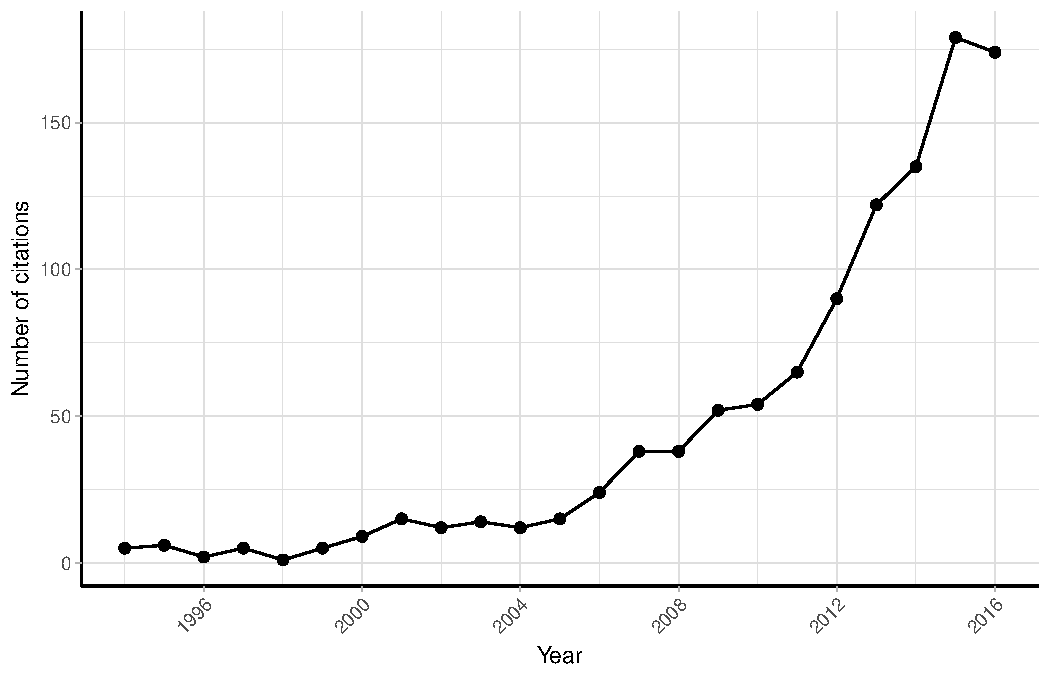
\includegraphics[width=\textwidth]{../figure/cite_grl-1} 

}

\caption[Number of citations of the paper by Greenland and Longnecker (1992) obtained from Google Scholar 1992-2017 (until December 2017)]{Number of citations of the paper by Greenland and Longnecker (1992) obtained from Google Scholar 1992-2017 (until December 2017).}\label{fig:cite_grl}
\end{figure}


\end{knitrout}

The most popular fields of application include oncology, public environmental and public health, nutrition epidemiology, and general internal medicine. Dose-response meta-analyses are published in many leading medical and epidemiological journals, including JAMA, Lancet, Stroke, Gastroenterology, American J of Medicine, American J of Clinical Nutrition, American J Epidemiology, International J Epidemiology, Journal National Cancer Institute, International J of Cancer, Statistics in Medicine and many others. The method is also used by the World Cancer Research Fund/American Institute for Cancer Research for reviewing the evidence on the relations between life-style factors (e.g. diet and physical activity) and cancer. Guidelines based on these quantitative reviews are central to promote the overall health and prevent many chronic diseases.

The common approach for dose--response meta-analysis consists of a two-stage procedure, where the regression coefficients for the study-specific trends are first estimated separately within each study, and then combined using meta-analysis. In the next sections we cover the main methodological aspects related to each stage of the analysis.


\subsection{First stage: study-specific trends}

If we had access to the individual patient data, the dose-response model for a simple linear trend could be written as
\begin{equation}
\log \left( \lambda \left(x, \mathbf{z} \right) \right) =  \beta_0 + \beta_1x + \boldsymbol{\gamma}^\top \mathbf{z}
\label{eq:lin_ipd}
\end{equation}
\noindent with $x$ the quantitative exposure and $z$ the set of possible confounders. The outcome variable is the log of a transformation of the mean outcome (e.g. odds, risk, or rate). Transformations of the exposure variable can be included to relax the linearity assumption, such as a quadratic term
\begin{equation}
\log \left( \lambda \left(x, \mathbf{z} \right) \right) =  \beta_0 + \beta_1x + \beta_2x^2 + \boldsymbol{\gamma}^\top \mathbf{z}
\label{eq:quadr_ipd}
\end{equation}
\noindent However, we have rarely access to the individual patient data and our inference is limited to a summary of the initial data. In particular, aggregated data from a categorical analysis can be often retrieved from published articles. 
\noindent The aim of the first stage of a dose--response meta-analysis is to estimate the $\beta$ coefficients in equation \ref{eq:lin_ipd} and \ref{eq:quadr_ipd} using aggregated dose--response data. We consider the notation presented in table~\ref{tab:aggr_data} with $i = 1, \dots, I$ indexing the studies and $j = 1, \dots, J_i$ the non-referent dose levels of a generic $i$-th study. The corresponding two models can be written as
\begin{equation}
\log \left( \widehat{\mathrm{RR}}_{ij} \right) = \log \left( \hat \lambda \left(x = x_{ij} \right) \right) - \log \left( \hat \lambda \left(x = x_{i0} \right) \right) = \beta_1\left(x_{ij} - x_{i0} \right)
\label{eq:lin_ad}
\end{equation}
\begin{equation}
\log \left( \widehat{\mathrm{RR}}_{ij} \right) = \log \left( \hat \lambda \left(x = x_{ij} \right) \right) - \log \left( \hat \lambda \left(x = x_{i0} \right) \right) = \beta_1\left(x_{ij} - x_{i0} \right) + \beta_2\left(x_{ij}^2 - x_{i0}^2 \right)
\label{eq:quadr_ad}
\end{equation}

\noindent More generally, the $i$-th dose-response model is defined as
\begin{equation}
\mathbf{y}_i = \mathbf{X}_i \boldsymbol{\beta}_i + \boldsymbol{\varepsilon}_i
\label{eq:drmodel}
\end{equation}
The outcome $\mathbf{y}_i $ is the $J_i$ length vector of the non-referent log $\widehat{\mathrm{RR}}$s while $\mathbf{X}_i$ the $J_i \times p$ design matrix containing the $p$ transformations of the assigned dose used to model the dose--response association
\begin{equation}
 \mathbf{X}_i=\left[
\begin{array}{ccc}
g_{1}(x_{i1}) - g_{1}(x_{i0}) & \hdots & g_{p}(x_{ip}) - g_{p}(x_{i0}) \\
\vdots &  & \vdots \\
g_{1}(x_{iJ_i}) -  g_{1}(x_{i0}) & \hdots & g_{p}(x_{iJ_i}) -  g_{p}(x_{i0}) \\
\end{array}%
\right] 
\label{eq:des.matrix}
\end{equation}

\noindent In the linear trend analysis (model~\ref{eq:lin_ad}), $\mathbf{X}_i$ includes only the dose levels, $p$ = 1, $g_1(x) = x$ (identity function)

\begin{equation*}
 \mathbf{X}_i=\left[
\begin{array}{c}
x_{i1} - x_{i0} \\
\vdots \\
x_{iJ_i} - x_{i0} \\
\end{array}%
\right] 
\end{equation*}

\noindent while $p = 2$ columns are needed in the quadratic model ~\ref{eq:quadr_ad}: $g_1(x) = x$ and $g_2(x) = x^2$

\begin{equation*}
 \mathbf{X}_i=\left[
\begin{array}{cc}
x_{i1} - x_{i0} & x_{i1}^2 - x_{i0}^2 \\
\vdots & \vdots \\
x_{iJ_i} - x_{i0} & x_{iJ_i}^2 - x_{i0}^2 \\
\end{array}%
\right] 
\end{equation*}

\noindent A feature of the models \ref{eq:drmodel} is the absence of the intercept term. The reference line in table~\ref{tab:aggr_data} is not actually used for the estimation of the regression coefficients but introduces the constrain on the predicted log $\widehat{\mathrm{RR}}$, which needs to be 0 ($\widehat{\mathrm{RR}}$ = 1) for the reference dose value $x_{i0}$, as explicit in models~\ref{eq:lin_ad} and~\ref{eq:quadr_ad}.

\subsubsection*{Approximation of the covariance between log $\widehat{\mathrm{RR}}$}

\noindent A particular characteristic of summarized dose--response data is that the log $\widehat{\mathrm{RR}}$s are reported with different precision and are constructed using the same baseline group. Thus, the error terms $\boldsymbol{\varepsilon}_i$ in equation~\ref{eq:drmodel} are heterogeneous and correlated, with a covariance matrix structured as
\begin{equation}
\Cov\left(\boldsymbol{\epsilon}_i\right) = \mathbf{S}_i = \left[
\begin{array}{ccccc}
\sigma_{i11} & \ \ & \ & & \ \\
\vdots \ & \ddots & & & \ \\
\sigma_{i1j}& \ & \sigma_{ijj}& & \ \\
\vdots & \ & \ & \ddots & \\
\sigma_{i1J_i} & \ldots & \sigma_{iJ_ij} & \ldots & \sigma_{iJ_iJ_i}
\end{array}
\right] 
\label{eq:S_i}
\end{equation}
\noindent with the variance of the log $\widehat{\mathrm{RR}}$s on the diagonal ($\sigma_{ijj}$) and the pairwise covariances as non-diagonal elements ($\sigma_{ijj'}$).

Two methods have been proposed to approximate the covariances $\sigma_{ijj'}$ \citep{greenland1992methods, hamling2008facilitating}. Greenland and Longnecker described an algorithm to construct a table of pseudo or effective counts (number of cases and participants or person-time) that would produce the adjusted log $\widehat{\mathrm{RR}}$s as those published. A unique solution for the algorithm is ensured by keeping the margins of the pseudo-counts equal to the observed ones. Alternatively, Hamling et al. modified the previous algorithm in such a way that the pseudo-counts would also match the standard errors of the log $\widehat{\mathrm{RR}}$s. Negligible differences in the reconstructed covariance matrices were found when comparing the two methods \cite{orsini2011meta}.

\subsubsection*{Estimation}

The dose-response coefficients $\boldsymbol{\beta}_i$ can be efficienly estimated using generalized least squares estimator (GLS), which minimizes the quadratic loss function $\left(\mathbf{y}_i- \mathbf{X}_i \boldsymbol{\beta}_i \right)^\top \mathbf{S}_i^{-1} \left(\mathbf{y}_i- \mathbf{X}_i \boldsymbol{\beta}_i \right)$ with respect to $\boldsymbol{\beta}_i$ assuming the covariance matrix $\mathbf{S}_i$ known. 
\begin{equation}
\begin{gathered}
\boldsymbol{\hat \beta}_i = ( \mathbf{X}_i^\top  \mathbf{S}_i^{-1} \mathbf{X}_i)^{-1} \mathbf{X}_i^\top  \mathbf{S}_i^{-1} \mathbf{y}_i \\ 
\widehat{\Var} \left( \boldsymbol{\hat \beta}_i \right) = ( \mathbf{X}_i^\top \mathbf{S}_i^{-1} \mathbf{X}_i)^{-1}
\end{gathered}
\label{eq:gls}
\end{equation}

\noindent The GLS estimates in equation~\ref{eq:gls} do not require any distributional assumption for the error terms. However, for the central limit theory, the error terms follow approximately a normal distribution $\boldsymbol{\epsilon}_i \sim \mathcal{N}\left(\mathbf{0}, \mathbf{S}_i \right)$. 
Using this additional assumption, the log-likelihood of model~\ref{eq:drmodel} is
\begin{equation}
\ell\left(\boldsymbol{\beta}_i\right) = -\frac{J_i}{2}\log\left(2\pi\right) - \frac{1}{2}|\mathbf{S}_i| - \frac{1}{2} \left[\left(\mathbf{y}_i- \mathbf{X}_i \boldsymbol{\beta}_i \right)^\top \left( \mathbf{S}_i \right)^{-1} \left(\mathbf{y}_i- \mathbf{X}_i \boldsymbol{\beta}_i \right) \right]
\label{eq:drmodel_logLik}
\end{equation}

\noindent Interestingly, the maximum likelihood estimates that maximize the log-likelihood~\ref{eq:drmodel_logLik} coincides with the GLS estimates in~\ref{eq:gls} \citep{orsini2006generalized}. Introducing the normality distribution for the random errors facilitates the inference, i.e. test of hypothesis and confidence intervals, on the $\boldsymbol{\beta}_i$ coefficients. The estimates in~\ref{eq:gls} are a linear combination of normal distributions ($\mathbf{y}_i \sim \mathcal{N}\left(\mathbf{X}_i \boldsymbol{\beta}_i, \mathbf{S}_i \right)$) and therefore are also normally  distributed $\boldsymbol{\hat \beta}_i \sim \mathcal{N}\left( \boldsymbol{\beta}_i, {\Var} \left( \boldsymbol{\hat \beta}_i \right)\right)$.

The ML and GLS estimators always give unbiased estimates of $\boldsymbol{\beta}_i$ regardless of the specification of $\mathbf{S}_i$ \citep{orsini2006generalized}. As a consequence, also a weighted least square estimator (WLS) that assumes independence of the log $\widehat{\mathrm{RR}}$s will produce unbiased estimates. However, taking into account the correlation will improve the statistical properties of the estimator, in particular the efficiency. 
We investigated the differences between the GLS and WLS estimators using a simulation study of 5000 aggregated dose--response data where the true trends were linear ($\beta_\text{TRUE} =$ -0.014). As expected, both the estimators were unbiased and consistent but the empirical distribution of the GLS estimator was more concentrated around the true $\beta$ value \ref{fig:cov_methods_lin}. The WLS estimates of the standard errors of the $\hat \beta_i$ were lower than the corresponding GLS values. This had a direct effect on the inference for the estimated linear trend. For istance, it may be interesting to fit a quadratic curve as in~\ref{eq:quadr_ad} and test the hypothesis $H_0: \beta_2 = 0$, i.e. departure from a linear trend. Using inference based on WLS estimators the null hypothesis were wrongly rejected 3.96\% of the time, lower than the nominal level $\alpha = 5$\%. The corresponding number for the GLS estimator was instead closer (4.8\%). 
\noindent We also implemented simulations assuming a quadratic curve with the true coefficients $\boldsymbol{\beta}_\text{TRUE}$ = (-0.092, 0.003). Similar results for the empirical bivariate distribution of $ \boldsymbol{\hat \beta}_i$ and their standard errors are presented in figure~\ref{fig:cov_methods_quadr}.

\begin{knitrout}
\definecolor{shadecolor}{rgb}{0.969, 0.969, 0.969}\color{fgcolor}\begin{figure}[ht!]

{\centering \includegraphics[width=\textwidth]{../figure/cov_methods_lin-1} 

}

\caption[Empirical distribution of the $\hat \beta$ (panel A) and $\widehat{\Var} \left( \hat \beta_i \right)$ (panel B) for a linear trend assuming independence of the log $\widehat{\mathrm{RR}}$  and reconstructing the covariances using the Greenland and Longnecker’s method]{Empirical distribution of the $\hat \beta$ (panel A) and $\widehat{\Var} \left( \hat \beta_i \right)$ (panel B) for a linear trend assuming independence of the log $\widehat{\mathrm{RR}}$  and reconstructing the covariances using the Greenland and Longnecker’s method. Results are based on simulations with 5000 replications and a true linear trend $\beta = $-0.014.}\label{fig:cov_methods_lin}
\end{figure}


\end{knitrout}

\begin{knitrout}
\definecolor{shadecolor}{rgb}{0.969, 0.969, 0.969}\color{fgcolor}\begin{figure}[ht!]

{\centering \includegraphics[width=\textwidth]{../figure/cov_methods_quadr-1} 

}

\caption{Empirical bivariate distribution of the beta coefficients (panel A) and their standard errors (panel B) for a quadratic trend assuming independence of the log $\widehat{\mathrm{RR}}$  and reconstructing the covariances using the Greenland and Longnecker’s method. Results are based on simulations with 5000 replications and a true quadratic trend $\beta_{1} = $-0.092, $\beta_{2} = $0.003.}\label{fig:cov_methods_quadr}
\end{figure}


\end{knitrout}


\subsection{Second stage: multivariate meta-analysis}

The study-specific dose-response curves are defined by the $p$ transformations, $g_1(x), \dots, g_p(x)$, and the estimated regression coefficients $\boldsymbol{\hat \beta}_i$. A pooled dose--response can be obtained by combining the $\boldsymbol{\hat \beta}_i$ coefficients. For that purpose, the same functional relationship needs to be defined across the studies. Therefore, the transformations of the exposure were not subscripted by the study index $i$.

\noindent The $p$ length vector of the $\boldsymbol{\hat \beta}_i$ parameters and the accompanying $p \times p$ covariances matrices $\widehat{\Var} \left( \boldsymbol{\hat \beta}_i \right)$ serve as outcome in the meta-analytic model. We consider the more general setting with $p \ge 2$ and relate the univariate case as a simpler instance. Since the dimension of the outcome is no longer univariate, extensions of models \ref{eq:rma} to the multivariate settings can be implemented for accommodating the synthesis of correlated estimates.

\subsubsection*{Model definition}

A multivariate random-effects model has a similar formulation as in the univariate case
\begin{equation}
\boldsymbol{\hat \beta}_i = \boldsymbol{\beta} + \mathbf{u}_i + \boldsymbol{\varepsilon}_i
\label{eq:rmma}
\end{equation}
\noindent The unobserved random effects $\mathbf{u}_i$ are now of dimension $p$ representing study-specific deviation from the mean $\boldsymbol{\beta}$ parameter. As before, they have zero mean $\E\left[\mathbf{u}_i\right] = \mathbf{0}$ and $\Var\left[\mathbf{u}_i\right] = \boldsymbol{\Psi}$, the $p \times p$ between-study variance matrix. An additional distributional function for the random-effects may facilitate the inference (especially confidence intervals) and improve the prediction of marginal and conditional dose-response association. Typically a multivariate normal distribution is adopted $\mathbf{u}_i \sim \mathcal{N}\left(\mathbf{0}, \boldsymbol{\Psi} \right)$. Hence, we can write the marginal model of~\ref{eq:rmma} as
\begin{equation}
\boldsymbol{\hat \beta}_i \sim \mathcal{N}\left(\boldsymbol{\beta}, \boldsymbol{\Sigma}_i \right)
\label{eq:rmma2}
\end{equation}
\noindent where the marginal variance $\boldsymbol{\Sigma}_i = \widehat{\Var} \left( \boldsymbol{\hat \beta}_i \right) + \boldsymbol{\Psi}$ is defined by the sum of the within-study and between-studies variance components. The model~\ref{eq:rmma2} implies a two-stage sampling procedure where the study-specific $\boldsymbol{\beta}_i$ parameters are assumed to be sampled from a multivariate normal distribution centered around the population average parameter $\boldsymbol{\beta}$. The study-specific estimates $\boldsymbol{\hat \beta}_i$ are themselves sampled from a multivariate distribution with zero mean and error variance assumed known.

The multivariate random-effects model~\ref{eq:rmma2} can be extended to meta-regression models by including study-levels covariates that might change the shape of the dose-response relationship. The dose-response coefficients are modeled as a linear combination of the $m$ study-level covariates $\mathbf{z}_i = \left(z_{i1}, \dots, z_{im} \right)$, with $ 
z_{i1} = 1$ indicating the intercept term
\begin{equation}
\boldsymbol{\hat \beta}_i \sim \mathcal{N}\left(\mathbf{Z}_i\boldsymbol{\beta}, \boldsymbol{\Sigma}_i\right)
\label{eq:rmmra2}
\end{equation}
\noindent The $p\times pm$ design matrix $\mathbf{Z}_i$ is constructed taking the Kronecker between the $\mathbf{z}_i$ and the identity matrix of dimension $p$ ($\mathbf{I}_{(p)}$)
\begin{equation}
\mathbf{Z}_i = \mathbf{I}_{(p)} \otimes \mathbf{z}_i^\top = 
	\begin{bmatrix}
		1 & z_{i2} & \cdots & z_{im} & \cdots & 0 & 0 & \cdots & 0 \\
		\vdots &  &  &  & \ddots & &  &  &  \\
		0 & 0 & \cdots & 0 & \cdots & 1 & z_{i2} & \cdots & z_{im} \\
	\end{bmatrix}
\end{equation}
\noindent For example, the $\mathbf{Z}_i$ matrix relating the effect of a binary variable $z_i$ to the dose--response coefficients for a quadratic trend is
\begin{equation*}
\mathbf{Z}_i = \mathbf{I}_{(2)} \otimes \mathbf{z}_i^\top = 
	\begin{bmatrix}
		1 & 0 \\
		0 & 1
	\end{bmatrix} \otimes
	(1, z_i)=
	\begin{bmatrix}
		1 & z_i  & 0 & 0 \\
		0 & 0 & 1 & z_i  \\
	\end{bmatrix}
\end{equation*} 

\subsubsection*{Estimation}

Several methods are available for estimating the parameters of interest, namely the $p$ dose--response coefficients in $\boldsymbol{\beta}$ and the $p(p+1)/2$ length vector $\boldsymbol{\xi}$ containing the elements of the between-studies covariance $\boldsymbol{\Psi}$. There is generally no reason to assume a specific covariance structure. We consider here likelihood-based estimators \citep{verbeke1997linear, pinheiro2010mixed}. In particular, ML estimators estimates simultaneously $\boldsymbol{\beta}$ and $\boldsymbol{\xi}$ by maximizing the log-likelihood the marginal model~\ref{eq:rmmra2}
\begin{equation}
\ell\left(\boldsymbol{\beta}, \boldsymbol{\xi} \right) = -\frac{1}{2}Ip\log(\pi) -\frac{1}{2}\sum_{i=1}^I \log |\boldsymbol{\Sigma}_i| - \frac{1}{2}\sum_{i=1}^I\left[ \left(\boldsymbol{\hat \beta}_i - \mathbf{Z}_i\boldsymbol{\beta} \right)^\top \boldsymbol{\Sigma}_i^{-1} \left(\boldsymbol{\hat \beta}_i - \mathbf{Z}_i\boldsymbol{\beta} \right) \right]
\label{eq:rmma_logLik}
\end{equation}

\noindent ML estimators, however, don’t take into account the loss of degrees of freedom due to the $\boldsymbol{\beta}$ estimation. Alternatively, restricted maximum likelihood methods (REML) maximizes a set of contrasts defined as a function of the only covariance parameters
\begin{align}
\ell_R\left(\boldsymbol{\xi} \right) =& -\frac{1}{2}\left(Ip - pm\right) -\frac{1}{2}\sum_{i=1}^I \log |\boldsymbol{\Sigma}_i| -\frac{1}{2}\sum_{i=1}^I \log \left|\mathbf{Z}_i^\top\boldsymbol{\Sigma}_i\mathbf{Z}_i \right| + \\
&- \frac{1}{2}\sum_{i=1}^I\left[ \left(\boldsymbol{\hat \beta}_i - \mathbf{Z}_i\boldsymbol{\beta} \right)^\top \boldsymbol{\Sigma}_i^{-1} \left(\boldsymbol{\hat \beta}_i - \mathbf{Z}_i\boldsymbol{\beta} \right) \right]
\label{eq:rmma_logRLik}
\end{align}

\noindent Both estimation methods require iterative algorithms, where conditional estimates of $\boldsymbol{\hat \beta}$ are plugged in either \ref{eq:rmma_logLik} or \ref{eq:rmma_logRLik}, regarded as function of $\boldsymbol{\xi}$ only, until convergence.

\subsubsection*{Hypothesis testing and heterogeneity}

There are two main domains of interest for making inference on the parameters that relate either to the fixed-effects $\boldsymbol{\beta}$ or the variance components in $\boldsymbol{\Psi}$. Using the normality assumption for the random-effects, inference is based on the approximated normal distribution for $\boldsymbol{\hat \beta}$, with mean and covariance matrix defined similarly as in equation~\ref{eq:gls}.

\noindent Since the mean dose-response association is defined by the $\boldsymbol \beta$, the hypothesis of no association can be evaluated by testing $H_0: \boldsymbol{\beta} = \boldsymbol{0}$. 
%In case of $p > 1$ multivariate Walt-type test are needed.
Alternatively, a subset or linear combinations of $\boldsymbol \beta$ may be interesting. For example, in a quadratic trend the non-linearity is introduced by the quadratic term $x^2$. Thus, testing $H_0: \beta_2 = 0$ is a possible way for evaluating departure from a linear dose-response relationship.

As previously presented in section~\ref{sec:het_rma}, the coefficients defining $\boldsymbol{\Psi}$ are not nuisance parameters rather than useful for quantifying the variation of the study-specific associations $\boldsymbol{\beta}_i$. Similar measures of testing and quantifying the impact of heterogeneity have been extended to the multivariate setting. In particular, the $Q$~statistic
\begin{equation}
Q = \sum_{i=1}^I \left(\boldsymbol{\hat \beta}_i - \mathbf{Z}_i\boldsymbol{\hat \beta}_{\text{fe}}\right) ^\top \widehat{\Var} \left( \boldsymbol{\hat \beta}_i \right)^{-1} \left(\boldsymbol{\hat \beta}_i - \mathbf{Z}_i\boldsymbol{\hat \beta}_{\text{fe}}\right)
\label{eq:Qmulti}
\end{equation}
\noindent with $\boldsymbol{\hat \beta}_{\text{fe}}$ estimating under a fixed-effect model, is used to test $H_0: \boldsymbol{\Psi} = \boldsymbol{0}$. Under the null hypothesis, the $Q$~statistic follow a $\chi^2$ with $Ip - pm$ degrees of freedom. When $p = 1$ the formulations~\ref{eq:Q} and~\ref{eq:Qmulti} coincide. The multivariate extension of the $I^2$ was derived relating the $Q$~statistics to its degrees of freedom $I^2 = \max \left\{0, \frac{Q- (Ip - pm)}{Ip - pm}\right\}$.

\subsubsection*{Prediction}

Oftentimes the estimated mean coefficients $\boldsymbol{\hat \beta}$ are not directly interpretable (an exception is the estimate for a linear trend). The dose-response results are thus communicated as predicted (log) relative risk for selected exposure levels using one value as referent. Obtaining predictions either in a graphical or tabular presentation is thus an important step of the analysis and yet often poorly implemented.

Based on the model~\ref{eq:rmma}, the predicted $\log RR$ for a dose level $x_v$ using $x_\mathrm{ref}$ as referent can be calculated as
\begin{align}
\log \widehat{RR}(x = x_v) = \left(\mathbf{X}_v\boldsymbol{\hat \beta} \right) \label{eq:pred} \\
\Var \left(\log \widehat{RR}(x = x_v) \right) = \mathbf{X}_v \widehat{\Var} \left( \boldsymbol{\hat \beta} \right) \mathbf{X}_v^\top \label{eq:varpred}
\end{align}
\noindent where $\mathbf{X}_v$ is the design matrix defined in the first-stage analysis (equation~\ref{eq:des.matrix}). For example, the predicted $\log RR$ for the quadratic model~\ref{eq:quadr_ad} comparing $x_v$ versus $x_\mathrm{ref}$ is
\begin{equation*}
\log \widehat{RR}(x = x_v) = \hat \beta_1 \left(x_v - x_\mathrm{ref} \right) + \hat \beta_2 \left(x_v^2 - x_\mathrm{ref}^2 \right)
\end{equation*}
Of note, the referent dose $x_\mathrm{ref}$ is an arbitrary value and thus does not need to correspond to any of the study-specific reference values $x_{i0}$.

\noindent A confidence interval for the predicted $\log \widehat{RR}(x = x_v)$ is based on the normal distribution of $\boldsymbol{\hat \beta}$
\begin{equation*}
\log \widehat{RR}(x = x_v) \mp z_{1- \alpha/2} \Var \left(\log \widehat{RR}(x = x_v) \right)^{\frac{1}{2}}
\label{eq:pred_ci}
\end{equation*}


Formulas~\ref{eq:pred} and~\ref{eq:varpred} can be extended to meta-regression models. The predicted $\log RR$ conditional on a specific study-level covariate pattern $\mathbf{z} = \mathbf{z}_v$ is
\begin{align}
\log \widehat{RR}\left(x = x_v, \mathbf{z} \right) = \mathbf{z}_v) = \left(\mathbf{X}_v \left(\mathbf{I}_{(p)} \otimes \mathbf{Z}_v^\top \right) \boldsymbol{\hat \beta} \right) \label{eq:pred_mr} \\
\Var \left(\log \widehat{RR}\left(x = x_v, \mathbf{z} \right) \right) = \left( \mathbf{X}_v \mathbf{Z}_v\right) \widehat{\Var} \left( \boldsymbol{\hat \beta} \right) \left( \mathbf{X}_v \mathbf{Z}_v\right)^\top \label{eq:varpred_mr}
\end{align}


\subsection{Methodological research}

Dose--response meta-analysis has received attention not only in applied works but also in theoretical articles that covered different aspects of the methodology. 
\noindent Greenland and Longnecker originally presented the two-stage approach for efficiently estimating a linear trend in a fixed-effect analysis. An alternative model for estimating curvilinear model, referred to as ``pool first'', was also presented. The technique consists of a one-stage approach where the aggregated data are considered altogether and a single model as in~\ref{eq:drmodel} is fitted. By first combining the data, more flexible curve such as polynomials or splines can be estimated. The study-specific dose-response analyses are limited by the minimum number of non-referent log RRs across the studies. For example, if the aggregated data for a study consists of only one non referent log RR, only a univariate model with $p = 1$ can be estimated. 
\noindent The authors refined the methodology by extending the two-stage approach to allow for heterogeneity for estimating a linear trend \citep{berlin1993meta}. In addition, they discussed alternatives for assigning the dose levels within exposure categories and presented meta-regression models to investigate the possible effect of study-level characteristics on the estimated linear trends. 

\subsubsection*{Flexible dose--response models}

The primary interest of the methodologicaln reserach was in presenting alternative strategies for estimating non-linear curves. Bagnardi et al. described the use of fractional polynomials and restricted cubic splines using aggregated dose--response data \citep{bagnardi2004flexible}. Based on a practical example on the association between alcohol consumption and all-cause mortality, the authors showed how implementation of these flexible techniques may prevent misleading results from conventional polynomials (e.g. quadratic) curves. Fractional polynomials of order two consist of large family of curves defined in the general form of
\begin{equation}
\mathrm{FP2}(x) = \beta_1 x^{p_1} + \beta_2x^{p_2}
\label{eq:fracpol}
\end{equation}
\noindent where $p_1$ and $p_2$ are chosen in the set of power coefficients $\left\{-2, -1, -0.5, 0, 0.5, 1, 2, 3 \right\}$. When $p = 0$ $x^p$ becomes $\log(x)$, while if $p_1 = p_2$ the second transformation of $x$ becomes $x^{p_2}\log(x)$. The advantage of models as in~\ref{eq:fracpol} is that different shapes, including U- and J-shapes, can be estimated by only two coefficients chosen using different combinations for the power terms $(p_1, p_2)$. Typically, the best fitting fractional polynomial is chosen in such a way that the $(p_1, p_2)$ corresponds to the model with the highest likelihood, or equivalently, lowest deviance. 

A popular alternative for flexibly model the dose--response association is represented by the use of splines, largely presented by Orsini et al. using data from the Pooling Project of Prospective Studies of Diet and Cancer \citep{orsini2011meta}. Splines functions consist of consecutive polynomials connected at specific points of the exposure range called knots. Choosing $\mathbf{k} = \left(k_1, \dots, k_K\right)$ knots and third order polynomials, also known as cubic splines (CS), the model is
\begin{equation}
\mathrm{CS}(x) = \beta_1 x + \beta_2x^2 + \beta_3x^3 + \sum_{l = 1}^{K-1} \beta_{l+3}(x - k_l)_{+}^3
\label{eq:cs}
\end{equation}
\noindent where the `+' notation has been used ($u_+ = u$ if $u \ge 0$ and $u_+ = 0$ otherwise). To avoid strange behaviors at the extremes of the exposure range, the model~\ref{eq:cs} is constraint to be linear before and after the first and last knots, respectively. For example, using three knots a restricted cubic spline model (RCS) is defied as
\begin{equation}
\mathrm{RCS}(x) = \beta_1 x + \beta_2 \left[ \left( x - k_1 \right)_{+}^3 - \frac{k_3 - k_1}{k_3 - k_2} \left( x - k_2  \right)_{+}^3 + \frac{k_2 - k_1}{k_3 - k_2} \left(x - k_3 \right)_{+}^3\right]
\label{eq:rcs}
\end{equation}
\noindent The second transformation is generally divided by $(k_3 - k_1)^2$ to improve the numerical behavior and to put the spline transformations on the same scale \citep{harrell2015regression}.

The previous strategies have been often presented for exposures where 0 was the natural reference categories (e.g. alcohol consumption). Liu et al. extended the methodology for handling non-zero reference categories, as in the case of Body Mass Index. In particular, they first described how to construct the design matrix in terms of contrasts, as clarified in equation~\ref{eq:des.matrix}. Misspecification of the design matrix (i.e. $\log \mathrm{RR} = \beta_1 (x_1 - x_0) + \beta_2 (x_1 - x_0)^2$ instead of $\log \mathrm{RR} = \beta_1 (x_1 - x_0) + \beta_2 (x_1^2 - x_0^2)$) may increase the risk of generating artifacts and misleading conclusions. Note that for zero exposure categories the problem is generally not relevant since many functions return zero for $x = 0$ ($g(0) = 0$).


\subsubsection*{Multivariate meta-analysis}

The major contribution for estimating non-linear curves in a random-effects analysis came with the extension of univariate meta-analytic models to the multivariate case. The formalization and implementation of multivariate meta-analysis enabled the extension of a two-stage dose--response meta-analysis to the more complex case of multiple parameters association \citep{gasparrini2012multivariate}. The multivariate framework can accommodate the synthesis of correlated outcomes, or estimates, derived in the first stage dose--response analyses. The application of the strategies presented in~\ref{eq:fracpol} and~\ref{eq:rcs} in a random-effects setting has been easily facilitated by the implementation of dedicated packages for multivariate meta-analysis \citep{orsini2011meta, jackson2011multivariate}.

\noindent More generally, the methodological advancements for meta-analysis were diverse and numerous (see \cite{sutton2008recent} for an overview). Important improvements that directly affected how results are presented related mainly to the quantification and assessment of hetereogenity, with the definition of the measures presented in~\ref{sec:het_rma}. In addition, many other articles enriched the set of tools for pooling study-specific effects, with a direct application to the second stage of a dose--response meta-analysis. Among the many, it is worth to mention the implementation of several estimation methods for the between-study variability (see for a comparison based on simulation studies); advancement in performing meta-regression; proposal of sequential approaches and statistical power; and introduction of Bayesian methods.



\subsection{Research questions}






\newpage

\section{Software}

\begin{knitrout}
\definecolor{shadecolor}{rgb}{0.969, 0.969, 0.969}\color{fgcolor}\begin{figure}[ht!]

{\centering \includegraphics[width=\textwidth]{../figure/dosresmeta_ts-1} 

}

\caption[Monthly number of downloads of the dosresmeta R package from the RStudio CRAN mirror September 2013 - December 2017]{Monthly number of downloads of the dosresmeta R package from the RStudio CRAN mirror September 2013 - December 2017.}\label{fig:dosresmeta_ts}
\end{figure}


\end{knitrout}

\begin{knitrout}
\definecolor{shadecolor}{rgb}{0.969, 0.969, 0.969}\color{fgcolor}\begin{figure}[ht!]

{\centering \includegraphics[width=\textwidth]{../figure/dosresmeta_map-1} 

}

\caption[Total number of downloads of the doseresmeta R package worldwide from the RStudio CRAN mirror September 2013 - December 2017]{Total number of downloads of the doseresmeta R package worldwide from the RStudio CRAN mirror September 2013 - December 2017.}\label{fig:dosresmeta_map}
\end{figure}


\end{knitrout}

% !TeX root = ../kappa.Rnw  


% ---------------------------------------------------------
% Project: PhD KAPPA
% File: aims.tex
% Author: Alessio Crippa
% based on the template written by Andrea Discacciati
%
% Purpose: Aims
% ---------------------------------------------------------

\chapter{Aims of the thesis}

The overall aims of this thesis were to develop and implement new methods for dose--response in meta-analysis, in order to deal with the methodological aspects that have not yet been addressed.

\bigskip

More specifically, the aims were:

\begin{itemize}
\item To describe the implementation of the main aspects of a dose--response meta-analysis and the usage of the \texttt{dosresmeta} $\R$ package.

\item To present and discuss relevant measures and graphical tools to assess the goodness-of-fit in dose--response meta-analysis.

\item To develop a new measure of between-study heterogeneity in the broader context of meta-analysis and assess its properties as compared to other available measures. 

\item To explore possible advantages of a point-wise approach, especially, in case of dose--response meta-analysis where the exposure range varies substantially across the studies.

\item To formalize and present an alternative one-stage random-effects model for dose--response meta-analysis of aggregated data, formulating the meta-analytic model in terms of a general linear mixed-effect model. 

\end{itemize}

% !TeX root = ../kappa.Rnw  


% ---------------------------------------------------------
% Project: PhD KAPPA
% File: materials.tex
% Author: Alessio Crippa
% based on the template written by Andrea Discacciati
%
% Purpose: Materials
% ---------------------------------------------------------

\chapter{Methods}

\section{The \texttt{dosresmeta} R package}

\subsection{Implementation}

\subsection{Exposure modeling}


\section{A new measure of heterogeneity}

\subsection{Statistical proporties}

\subsection{Simulation study}


\section{Goodness-of-fit}

\subsection{Deviance}

\subsection{Coefficient of determination}

\subsection{Visual tools}


\section{A point-wise approach}

\subsection{Prediction of study-specific (log) relative risks}

\subsection{Pool of dose--response prediction}


\section{A one-stage model}

\subsection{Model definition}

\subsection{Estimation and hypothesis testing}

\subsection{Prediction}

\subsection{Comparison with two-stage analysis}

% !TeX root = ../kappa.Rnw  

% ---------------------------------------------------------
% Project: PhD KAPPA
% File: results.tex
% Author: Alessio Crippa
% based on the template written by Andrea Discacciati
%
% Purpose: Results
% ---------------------------------------------------------

\chapter{Results}




% Paper I
%\input{results.1}

% !TeX root = ../kappa.Rnw  

% ---------------------------------------------------------
% Project: PhD KAPPA
% File: discussion.tex
% Author: Alessio Crippa
% based on the template written by Andrea Discacciati
%
% Purpose: Discussion
% ---------------------------------------------------------

\chapter{Discussion}

Write the discussion with subsections as in the background section

% !TeX root = ../kappa.Rnw  

% ---------------------------------------------------------
% Project: PhD KAPPA
% File: conclusions.tex
% Author: Alessio Crippa
% based on the template written by Andrea Discacciati
%
% Purpose: Conclusions
% ---------------------------------------------------------

\chapter{Conclusions}

The methods presented in this thesis enrich the set of tools available for applying dose--response meta-analyses and for addressing specific questions including how to evaluate the goodness-of-fit and how to measure the impact of the between-studies heterogeneity. Furthermore, this thesis describes alternative models for pooling results in case of heterogeneous exposure range and for estimating complex models without excluding relevant studies. The proposed methods have been illustrated using real data from published meta-analyses and implemented in the \texttt{dosresmeta} and \texttt{hetmeta} $\R$ packages available on CRAN. 

More specifically we conclude the following:

\begin{itemize}

\item The \texttt{dosresmeta} $\R$ package can help practitioners to conduct dose--response meta-analyses and to apply the methods presented in this thesis. Dedicated functions help to avoid pitfalls frequently encountered in published meta-analyses, such as definition of the design matrix and prediction of the pooled results (\citetalias{crippadosresmeta2016}).

\item Goodness-of-fit should be regularly evaluated in applied dose--response meta-analysis. The proposed solutions consist of descriptive measures to summarize the agreement between fitted and observed data (the deviance and the coefficient of determination), and graphical tools to visualize the fit of the model (decorrelated residuals-versus-exposure plot). These tools can be employed to identify systematic dose--response patterns and possible source of heterogeneity, and to support the conclusions in applied meta-analyses (\citetalias{discacciati2015goodness}).

\item The new measure of heterogeneity, $R_b$, quantifies the proportion of the variance of the pooled estimate attributable to the between-study heterogeneity. Contrary to the available measures of heterogeneity, it does not make any assumption about the distribution of the within-study error variances, nor does it require specification of a typical value for these quantities. Therefore, we recommend the use of the $R_b$ as preferred measure for quantifying the impact of heterogeneity (\citetalias{crippa2016new}). 

\item A point-wise strategy for dose--response meta-analysis does not require the specification of a unique model as in the traditional approaches, and therefore allows for more flexibility in modeling the individual curves. In addition, the extent of extrapolation is limited by predicting the study-specific relative risk based on the observe exposure range. The use of the described strategy may improve the robustness of the results, especially in case of heterogeneous exposure range (\citetalias{crippa2018pointwise}).

\item A one-stage approach for dose--response meta-analysis consists of a linear mixed-effects model, which offer useful tools for describing the impact of heterogeneity over the exposure range, for comparing the fit of different models, and for predicting individual dose--response associations. Thhe main advantage is that flexible curves can be estimated regardless of the number of data-points in the individual analyses (\citetalias{crippa2018one}).

\end{itemize}

% !TeX root = ../kappa.Rnw  

% ---------------------------------------------------------
% Project: PhD KAPPA
% File: future.tex
% Author: Alessio Crippa
% based on the template written by Andrea Discacciati
%
% Purpose: Future research
% ---------------------------------------------------------

\chapter{Future research}

Based on the conclusions presented in this thesis, future research includes: 

\begin{itemize}
\item <>

\item <>

\item <>
\end{itemize}

% Appendix
\appendix

% !TeX root = ../kappa.Rnw  

% ---------------------------------------------------------
% Project: PhD KAPPA
% File: appendix.tex
% Author: Alessio Crippa
% based on the template written by Andrea Discacciati
%
% Purpose: Appendix
% ---------------------------------------------------------

\chapter{Supplementary figures}

Figures.

%--tables
\chapter{Supplementary tables}

Tables.

% Back matter
\backmatter
\bibliographystyle{style/jss}
\refstepcounter{chapter}
\addcontentsline{toc}{chapter}{\bibname}
\bibliography{additional/kappa_bib}
\newpage
\pagestyle{nothing}

% ---------------------------------------------------------
% Project: PhD KAPPA
% File: acknowledgements.tex 
% Author: Alessio Crippa
% based on the template written by Andrea Discacciati
%
% Purpose: Acknowledgements
% ---------------------------------------------------------

\chapter{Acknowledgements}

There are many people that I would like to thank for their contributions to this thesis, and for their support and encouragement during these years.

\bigskip

\textbf{Nicola Orsini}, my main supervisor for the second half of my doctoral education.

\bigskip

\noindent This work was supported by \textbf{Karolinska Institutet}'s funding for doctoral students (KID-funding).







\end{document}
